
\section{Conclusiones}

\subsection{PageRank}
Este algoritmo resultó bastante sencillo de implementar, una gran parte del mismo fue la implementación de la matriz esparsa para mejorar tanto la performance espacial como la temporal en el cálculo del método de la potencia. \\
En cuanto a tiempos es bastante estable y podemos deducir bajo las pruebas realizadas que debería seguir siendo así para grafos aún más grandes. A contrapartida, la calidad si bien es muy buena para c$=$0.15, lo que confirma el comentario en el paper original, notamos que hay un trabajo grande por encima en los buscadores reales pero es un muy buen punto de partida. Nos referimos a posicionamiento por publicidad, eliminación de SPAM, etc.

\subsection{HITS}

Una parte importante sobre este algoritmo es que tarda mucho para nodos grandes, sin embargo no debemos olvidar que en su paper$[2]$ Kleinberg habla de que este algoritmo debe ser aplicado no sobre toda la red sin sobre un subconjunto de la misma ($\textit{root set}$) obtenido de una busqueda incial. Por lo tanto si acotamos el análisis a los grafos mas acotados podemos ver que el tiempo de computo es aceptable y hasta muy parecido al de page rank. 

\subsection{INDEG}

Este algoritmo es bastante simple y en una red chica y confiable puede llegar a valer. Es muy rápido y en caso de necesitar algún dato rápido, es muy fácil de implementar. Igualmente tiene mucho peso la confiabilidad, ya que es muy simple de crecer tu puntaje, simplemente comprando un lugar mínimo en la mayor cantidad de páginas posibles.

%  \begin{figure}[!htb]
% \begin{center}
%     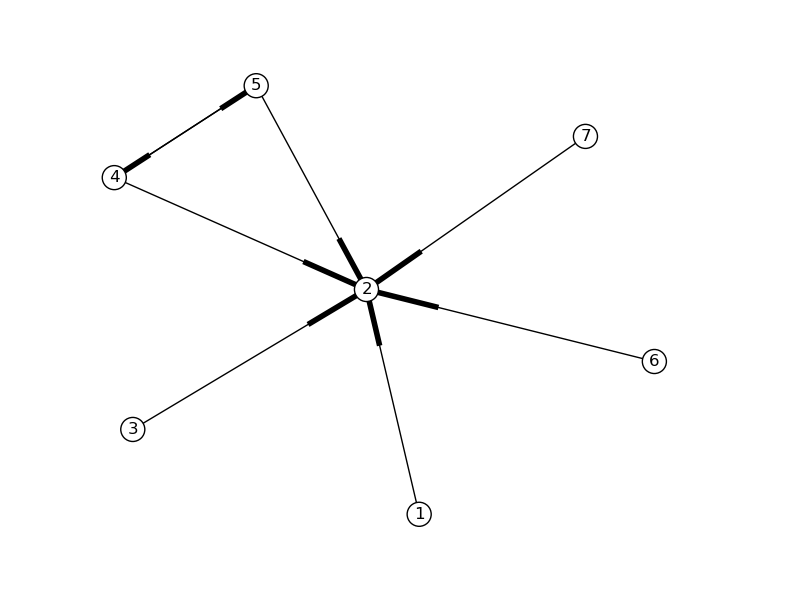
\includegraphics[scale=0.5]{imagenes/test4.png}
%     \caption{Red de 7 nodos}
%     \end{center}
% \end{figure}

% \subsection{Mejor estrategia para comprar links}
% \subsubsection{PageRank}

% Como explicamos anteriormente, el algoritmo de PageRank prioriza la calidad del sitio de entrada antes que la cantidad. Por lo tanto supongamos que tenemos el siguiente escenario:


%  \begin{figure}[!htb]
% \begin{center}
%     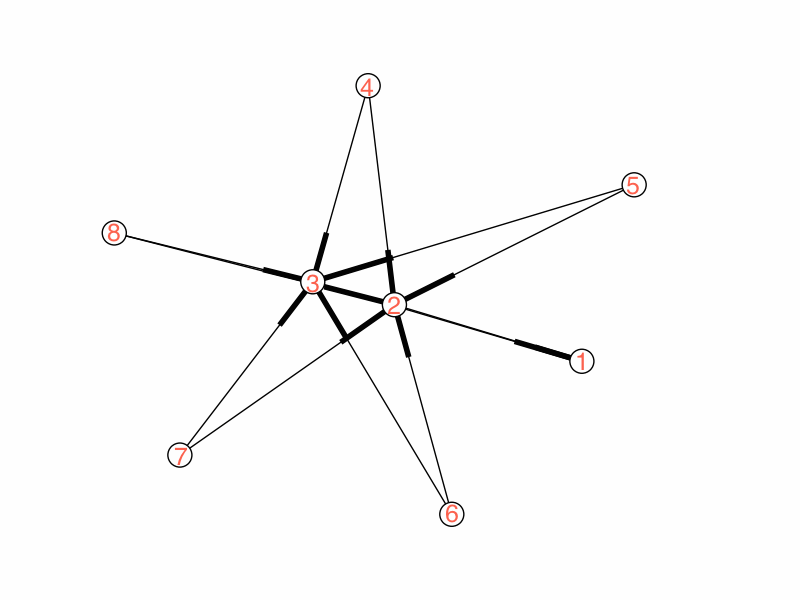
\includegraphics[scale=0.5]{imagenes/test6.png}
%     \caption{Red de 8 nodos, c=0.85}
%     \end{center}
% \end{figure}

% Cuyos pesos son:
%    $$ 
% \begin{bmatrix}
% Nodo 1 & 0.32079\\
% Nodo 2 & 0.15762\\
% Nodo 3 & 0.15762\\
% Nodo 4 & 0.05283\\
% Nodo 5 & 0.05283\\
% Nodo 6 & 0.05283\\
% Nodo 7 & 0.05283\\
% Nodo 8 & 0.05283\\
% \end{bmatrix} 
% $$

% Ahora, suponiendo que el costo de cada nodo es mas caro a medida que aumenta su peso, vamos a ver que es más conveniente, si comprar el derecho a que el nodo 1 nos apunte o en vez de eso comprar el linkeo de los nodos 2 y 3. Entonces vamos a testear como se comporta el algoritmo mediante estas dos alternativas lineando al sitio de los Wachiturros.


%    $$ 
% \begin{bmatrix}
%  & Nodo 1 & Nodo 2 y 3 \\
% Wachiturros & 0.24557  & 0.05018   \\
% Nodo 1 & 0.24201& 0.30469\\
% Nodo 2 & 0.11891& 0.14971\\
% Nodo 3 & 0.11891& 0.14971\\
% Nodo 4 & 0.03986  & 0.05018\\
% Nodo 5 & 0.03986  & 0.05018\\
% Nodo 6 & 0.03986  & 0.05018\\
% Nodo 7 & 0.03986 & 0.05018\\
% Nodo 8 & 0.03986 & 0.05018\\
% \end{bmatrix} 
% $$

% Por lo tanto se puede ver que conviene que el Nodo 1 nos apunte antes que el 2 y 3. Conviene porque nos asigna un mayor peso y porque nos deja a su vez mejor posicionado en la tabla final. Además de significar una optimización en el costo total.

\subsubsection{HITS}
Si el algoritmo aplicado en la red fuese HITS lo recomendable al cliente sería que negocie con los principales HUBS para que apunten a su sitio. Logrando así rankear mejor en la sección de Autoridades sobre el tema. 
No le recomendaríamos que negocie con las páginas autoridades ya que dificilmente estas accediesen debido a que de esta manera se estarían restando puntos en el ranking de autoridades.\\
Por ejemplo en el caso de death penalty habría que negociar con alguno de los 3 principales HUBS: clarkprosecutor.org, faculty.etsu.edu o coramnobis.com. Teniendo en cuenta el costo de cada uno, ya que si el primero costase el doble 
o mas que el segundo tal vez convendría más negociar con el segundo y tercero.
